\documentclass[crop,tikz]{standalone}

\usepackage{fontspec}
\setmainfont{texgyrepagella}[
  Extension = .otf,
  UprightFont = *-regular,
  BoldFont = *-bold,
  ItalicFont = *-italic,
  BoldItalicFont = *-bolditalic,
]

\usepackage{tikz}
\usetikzlibrary{decorations.pathreplacing,calligraphy}
\usetikzlibrary{calc}

\makeatletter % https://tex.stackexchange.com/a/38995/121799
\tikzset{
  use path/.code={\pgfsyssoftpath@setcurrentpath{#1}}
}
\makeatother
\tikzset{reverseclip/.style={insert path={(current bounding box.north
        east) rectangle (current bounding box.south west)}}}

\pgfdeclarelayer{bg}
\pgfsetlayers{bg,main}


\begin{document}

    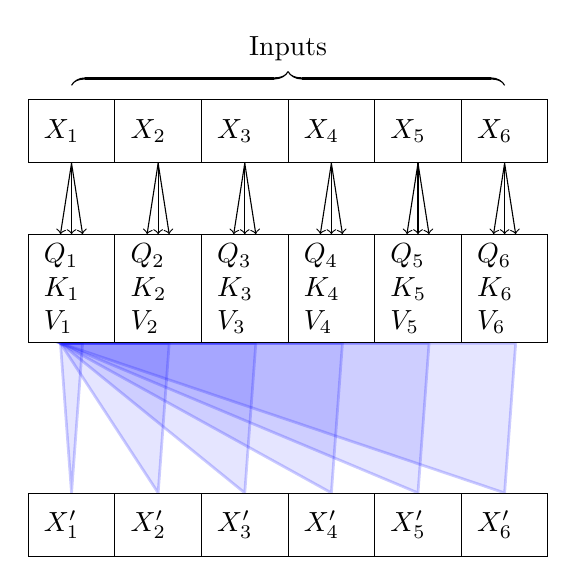
\begin{tikzpicture}
        \begin{scope}
            \tikzstyle{every node}=[draw,rectangle,text width=0.7cm, minimum width=1.1cm, minimum height=0.8cm]

            \begin{scope}[shift={(1.1cm * -3, 0)}]
                \foreach \x in {1,...,6} {
                    \node (i_\x) at (\x*1.1 cm, 0) {$X_{\x}$};
                }
                \begin{scope}[shift={(0, -2cm)}]
                    \foreach \x in {1,...,6} {
                        \node[transform shape,fill=white] (qkv_\x) at (\x*1.1 cm, 0) {$Q_{\x}$ $K_{\x}$ $V_{\x}$};
                        \draw[->] (i_\x.south) -- ([xshift=-4pt]qkv_\x.north);
                        \draw[->] (i_\x.south) -- (qkv_\x.north);
                        \draw[->] (i_\x.south) -- ([xshift=4pt]qkv_\x.north);
                    }
                \end{scope}
                \foreach \x in {1,...,6} {
                    \begin{scope}[shift={(0, -5cm)}]
                        \node[transform shape,fill=white] (y_\x) at (\x*1.1 cm, 0) {$X'_{\x}$};
                    \end{scope}
                    \begin{pgfonlayer}{bg}
                        \begin{scope}[
                        every path/.append style={draw=blue,fill=blue,fill opacity=0.1,draw opacity=0.2},
                        blend group=darken]
                            \fill[blue] (y_\x.north) -- ([xshift=-4pt]qkv_1.south) -- ([xshift=4pt]qkv_\x.south) -- cycle;
                        \end{scope}
                    \end{pgfonlayer}
                }
            \end{scope}
        \end{scope}

        \draw[thick,decorate,decoration={calligraphic brace,raise=5pt, amplitude=5pt}] (i_1.north) -- node[above=10pt] {Inputs} (i_6.north);

    \end{tikzpicture}

\end{document}
